\documentclass[12pt, a4paper]{report}
\usepackage[spanish]{babel}
\usepackage[utf8]{inputenc}
\usepackage{graphicx} 
\usepackage{amsmath}
\usepackage{algorithm}
\usepackage[noend]{algpseudocode}

\makeatletter
\def\BState{\State\hskip-\ALG@thistlm}
\makeatother

\graphicspath{ {images/} }

\title{%
Simulación de Sistemas\\
Trabajo Práctico 2: Autómata Celular Off-Lattice \\
\large Bandadas de Agentes Autopropulsados
}

\author{Piñeiro, Eugenia Sol - 59449\\
Baiges, Matías Sebastián - 59076\\
Comerci Wolcanyik, Nicolás - 59520
}
\date{3 de Septiembre de 2021}

\begin{document}

\maketitle

\tableofcontents
\newpage

\section{Introducción}
El objetivo del siguiente trabajo práctico es implementar un Autómata Celular \emph{Off-Latice}, 
a fin de analizar el comportamiento de partículas puntuales en base a distintos parámetros.\\

El autómata \emph{Off-Latice} se basa en un modelo matemático inspirado en el comportamiento colectivo de algunos Sistemas Naturales. Estos sujetos biológicos tienden a moverse con sus vecinos. Por ejemplo, bandadas, cardúmenes, manadas de cuadrúpedos o una colonia de bacterias.\\

En cuanto al sistema, las partículas se desplazan con velocidad absoluta constante. Las mismas, en cada paso de tiempo, asumen el promedio de las direcciones de las partículas vecinas de radio \emph{r} con un ruido añadido de forma aleatoria.\\

Este modelo exhibe un comportamiento cooperativo entre las partículas, las cuales a medida que va avanzando el tiempo comienzan a moverse con una simetría de forma espontánea.\\ 

La evolución temporal de las partículas viene dada por las siguientes ecuaciones: 
\begin{equation}
\label{eq:velocity}
x_i(t+1) = x_i(t) + v_i(t) \Delta t 
\end{equation}

donde \emph{x} es la posición de la partícula, \emph{v} la velocidad, y $\Delta$ \emph{t} el paso de tiempo  

\begin{equation}
\label{eq:angle}
\theta _i(t+1) = \left\langle \theta _i(t)\right\rangle _r + \Delta \theta 
\end{equation}
donde $\Delta \theta  \epsilon  [-\frac{\eta}{2}; \frac{\eta}{2}]$ es el ruido añadido, siendo $\eta$ la amplitud del ruido, y \emph{$\left\langle \theta _i(t)\right\rangle _r$} es el promedio de los ángulos de todas las partículas en un radio \emph{r}

\begin{equation}
\label{eq:avgangle}
\left\langle \theta _i(t)\right\rangle _r =  \frac{\left\langle sin(\theta _i(t))\right\rangle _r}{\left\langle cos(\theta _i(t))\right\rangle _r} 
\end{equation}

\section{Implementación}
La implementación del algoritmo \emph{Off-Lattice} se desarrolló en el lenguaje de programación \emph{Java}\\

El flujo principal del programa consiste en diversos pasos. En primer lugar, se obtienen los parámetros de configuración para iniciar la Simulación.\\

Luego, se generan partículas de forma aleatoria y se van actualizando tanto sus posiciones como sus ángulos con el algoritmo del autómata. \\

Por último, se guardan los resultados en distintos archivos que serán utilizados como \emph{input} para generar la Animación en \emph{Ovito} y realizar el postprocesamiento en \emph{Python} para hacer un análisis de resultados.\\

\begin{figure}[h]
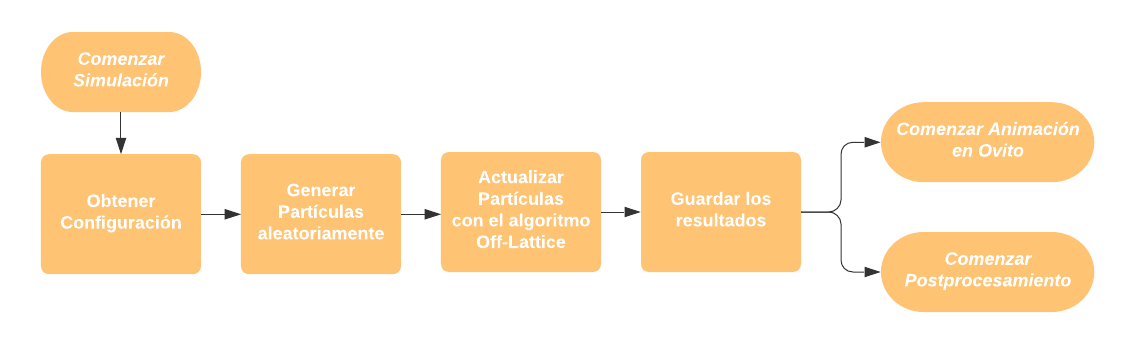
\includegraphics[scale=0.35]{Diagrama de flujo.png}
\centering 
\caption{Diagrama de Flujo}
\end{figure}

En cuanto a la implementación de la Simulación, se cuenta con distintas clases en Java. La clase que implementa el flujo principal (main) es \emph{OffLatticeSimulation}. Las partículas se modelaron con la clase \emph{VelocityPaticle}, que extiende de una clase \emph{Particle} y cuenta con su posición, ángulo y rapidez. Las mismas se generan a partir de la clase \emph{VelocityPartcileGenerator}.\\

Para calcular la polarización de las mismas se cuenta con la clase \emph{Polarization}. El algoritmo del autómata se implementó en la clase \emph{OffLattice} que hace uso de las mencionadas anteriormente.\\  

A su vez, se cuenta con las clases para obtener los parámetros de configuración y obtención de resultados \emph{Config, XYZWriter, JsonWriter} y \emph{Postprocessing}, sobre las cuales no se entrará en detalle ya que corresponden al postprocesamiento.

\pagebreak

\begin{figure}[h]
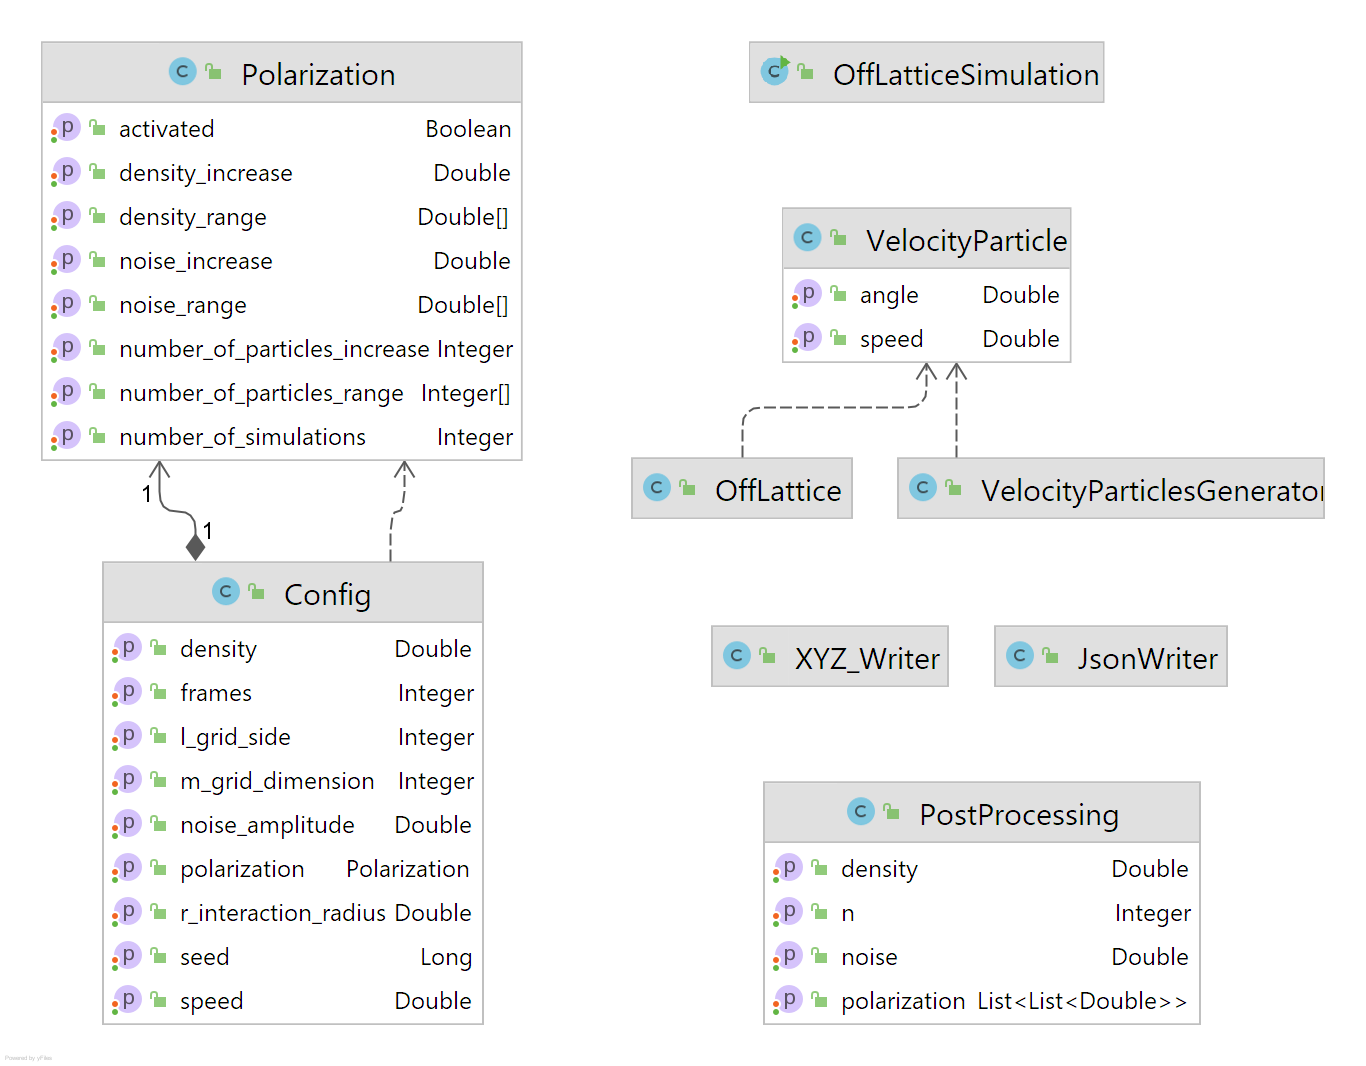
\includegraphics[scale=0.3]{UML.png}
\centering 
\caption{Diagrama de Flujo}
\end{figure}

A continuación se presentan los pseudocódigos correspondientes al flujo principal del programa y al algoritmo \emph{Off-Lattice}:

\pagebreak
\begin{algorithm}
    \caption{OffLattice Simulation Main}\label{main}
    \begin{algorithmic}[1]
    \Procedure{main}{}
    \State $\textit{config} \gets \text{mapper.readValues()}$
    \State $particles \gets \textit{VelocityParticlesGenerator.generateRandom(config)}$
    \State $frames \gets \textit{OffLattice.simulate(config)}$
    \State $XYZ_Writer(FILENAME).addAllFrames(frames)$
    \EndProcedure
    \end{algorithmic}
\end{algorithm}

\begin{algorithm}
    \caption{OffLattice Algorithm}\label{offLattice}
    \begin{algorithmic}[1]
    \Procedure{simulate}{}
    \BState \emph{\textbf{for} frame in frames}:
    \State $\textit{neighbours} \gets \text{CellIndexMethod.search()}$
    \BState \emph{\textbf{for} particle in neighbours + itself}:
    \State $\textit{newAngle} \gets \text{atan2(sinAvg, cosAvg) + noise}$
    \State $particle.setAngle(newAngle)$
    \State $particle.setCoords((x + speed * cos(newAngle)) \% L,(y + speed * sin(newAngle)) \% L)$
    \EndProcedure
    \end{algorithmic}
\end{algorithm}

\section{Simulaciones}

\subsection{Parámetros}

\section{Resultados}

\section{Conclusiones}




\end{document}